%Possible keys: sii, joc, cjm
\documentclass[sii]{ipart}
\pubyear{2014}
\volume{7}
\issue{0}
\firstpage{1}
\lastpage{}

\usepackage{natbib}
%\usepackage{hyperref}
\usepackage{bm}
\usepackage{subfigure}
\usepackage{amsmath, epsfig}
\usepackage{amsfonts}
\usepackage{graphicx} % for figures of all kinds
\graphicspath{{./figures/}}
%\arxiv{math.PR/0000000}

\begin{document}

\begin{frontmatter}

\title{Difficulty of selecting among multilevel models using predictive accuracy}
\runtitle{Selecting Multilevel Models}

\begin{aug}
  \author{Wei Wang\thanksref{t1}\ead[label=e1]{ww2243@columbia.edu}}
 \address{Department of Statistcs \\Columbia University\\ New York, New York
   10027\\ United States of America\\
          \printead{e1}}
        \and
 \author{Andrew Gelman\ead[label=e2]{gelman@stat.columbia.edu}}
 \address{Department of Statistcs and Political Science \\ Columbia
   University\\ New York, New York 10027\\ United States of America\\
          \printead{e2}}

\thankstext{t1}{Corresponding author.}
\runauthor{W. Wang and A. Gelman}
\end{aug}

\begin{abstract}
  As a simple and compelling approach for estimating out-of-sample prediction
  error, cross-validation naturally lends itself to the task of model
  comparison. However, even with moderate sample size, it can be surprisingly
  difficult to compare multilevel models based on predictive accuracy.  Using a
  hierarchical model fit to large survey data with a battery of questions, we
  demonstrate that even though cross-validation might give good estimates of
  pointwise out-of-sample prediction error, it is not always a sensitive
  instrument for model comparison.

\end{abstract}

\begin{keyword}[class=AMS] %please indicate appropriate AMS codes
\kwd[primary ]{62F15}
%\kwd{00K01}
\kwd[; secondary ]{62D05}
\end{keyword}

\begin{keyword}
\kwd{Multilevel Models}
\kwd{Predictive Accuracy}
\kwd{Model Selection}
\kwd{Sample Survey}
\kwd{Cross-Validation}
\end{keyword}

%\tableofcontents

\end{frontmatter}

% \title{\vspace{-.3in}}
% \date{\vspace{-.1in}8 Apr 2014\vspace{-.1in}}
% \author[1]{Wei Wang}
% \author[1,2]{Andrew Gelman}
% \affil[1]{Department of Statistics, Columbia University, New York}
% \affil[2]{Department of Political Science, Columbia University, New York}
% \maketitle
% %% So our target audience will be experts like people like David Dunson. We try to see how cross-validation works for

% % \nipsfinalcopy


\section{Introduction}

%% Why multilevel model is good for survey data?
%% Cross-Validation may not perform well for groups
%% What is cross-validation doing?

\subsection{Cross-validation for Hierarchical Models}

Cross-validation is a widely-used method for estimating out-of-sample prediction
error and comparison of statistical models. By fitting the model on the training data set and
then evaluating it on the testing set, the over-optimism of using data twice is
avoided. Furthermore,
attempts have been made to use cross-validated objective functions for
statistical inference \citep{craven1978smoothing, seeger2008cross}, thus
integrating out-of-sample prediction error estimation and model selection into
one step.

However, for multilevel data (as well as other dependent structures such as time
series, spatial, and network data), several challenges arise in the use of
cross-validation for estimating out-of-sample prediction error and model
selection. The first challenge is the lack of clear protocol for the
cross-validation procedure: to truly test the model, the holdout set cannot be a
simple random sample of the data but instead needs to have some multilevel
structure itself, so that entire groups as well as individual observations are
held out.  Hierarchical cross-validation can be performed in the context of
particular applications \citep{PriceGelmanNero:1996} but it is not clear how best
to subsample structured data for cross-validation in a general way.  The second
challenge is that, in multilevel models, the observed loss function for
data-level cross-validation can be so close to flat that the cross-validation
estimates of prediction errors under candidate models can be swamped by random
fluctuations.

We focus on the second of these concerns, demonstrating the limitations of
prediction error in the context of a set of multilevel models fit to a large
cross-tabulated national survey.  An innovative aspect of our analysis is that we
evaluate separately on 71 different survey responses, taking each in turn as the
outcome in a comparison of regression models.  This allows us to construct a
relatively large corpus of data out of a single survey.

Multilevel models are effective in survey research, as partial pooling can yield
accurate state-level estimates from national polls
\citep{gelman2007data}. Multilevel models have been successfully applied both to
representative and nonrepresentative surveys to obtain accurate small-area
estimation and prediction \citep{FayHerriot:1979, lax_2009, ghitza_2013,
  wang_2014}, and the practical application of such methods is currently being
actively discussed in social science research \citep{buttice_2013, lax_2013}. In
the present paper, we conduct model selection procedures based on $k$-fold
cross-validation and find that under this framework, the improvement of
multilevel models over classical models is surprisingly small when measured on
the scale of prediction error. Furthermore, we demonstrate that this lack of
notable improvement is related to the sample size and data structure by repeating
the analysis on simulated data sets that vary in terms of these two factors.

Our results illustrate that under multilevel structure, it could be tricky to
use cross-validation in model selection, as the size of the data and how balanced
the structure is heavily affect the relative performance of the models.

% Our results suggest that researchers should be cautious in using and
% interpreting cross-validation-based model selection in the presence of
% multilevel structure.


\subsection{Order of Magnitude Analysis of Prediction Errors in Binary-data Regressions}

What sorts of improvements in terms of expected predictive loss can we expect to
find from improved models applied to public opinion questions?  We can perform a
back-of-the-envelope calculation. Consider one cell with true proportion 0.4 and
three fitted models, a relatively good one that gives a posterior estimate of
0.41 and two poorer models that give estimates of 0.44 and 0.38.  The predictive
log loss is $-[0.4\,\log(0.41)+0.6\,\log(0.59)]=0.6732$ under the good model and
$-[0.4\,\log(0.44)+0.6\,\log(0.56)]=0.6739$ and
$-[0.4\,\log(0.38)+0.6\,\log(0.62)]=0.6763$ under the others.

In this example, the improvement in predictive loss by switching to the better model is between 0.0006 and
0.003 per observation. The lower bound is given by
$-[0.4\,\log(0.4)+0.6\,\log(0.6)]=0.6730$, so the potential gain from moving to
the best possible model in this case is only 0.0002.

These differences in expected prediction error are tiny, implying that they would
hardly be noticed in a cross-validation calculation unless the number of
observations in the cell were huge (in which case, no doubt the analysis would be
more finely grained and there would not be so many data points per cell).  At the
same time, a change in prediction from 0.38 to 0.41, or from 0.41 to 0.44, can be
meaningful in a political context.  For example, Mitt Romney in 2012 won 38\% of
the two-party vote in Massachusetts, 41\% in New Jersey, and 44\% in Oregon;
these differences are not huge but they are politically relevant, and we would
like a model to identify such differences if it is possible from data.

The above calculations are idealized but they gives a sense of the way in which real
differences can correspond to extremely small changes in predictive loss for
binary data.

% present some theoretical derivations on model selection based on prediction
% error, thus clarifying the estimands. Second, we propose a reasonable protocol
% for conducting $k$-fold cross-validation for data with deep hierarchical
% structure, and briefly discuss other alternatives. Third, we present the results
% on the survey data set and demonstrate the general difficulty of
% cross-validation as a model selection procedure when applied to multilevel data.

% Multilevel/Hierarchical modeling is widely used to analyze data sets
% with group structure.\citet{ARM} The central idea is to induce correlation between
% effects in different groups through introducing prior distributions on the
% parameters, which would otherwise be modeled in two discrete options, either as
% distinct or identical. For example, in analyzing the effect of income on voting
% preferences in all states of US, multilevel modeling allows the effect in New
% York to borrow strength from the effect estimated in Texas, but differ. This is
% also known as ``partial pooling'' feature of multilevel models. The prediction
% based on multilevel models, which can be interpreted as posterior point estimator
% from a Bayesian perspective or Best Linear Unbiased Predictor from a frequentist
% perspective, are known to have better property than prediction made from
% traditional approaches.

% The demonstrative data set used in this paper is the 2006 Cooperative
% Congressional Election Survey. Large survey data sets with a number of
% categorical variables present themselves in cross-tabulated form. Assuming all
% variables in the data set are categorical, survey data sets can be recast as a
% multi-way table. Data analysts are facing the dire options of either not including or
% selectively including the vast amount of possible interactions, which amounts to
% an additive model on group structures, or including full interactions,
% which amounts to fitting a completely separate model for each cell. Apparently,
% neither approach seems satisfactory.
% For example, in a political opinions survey, each cell
% represents the number of respondents, in a certain subpopulation, who hold a
% certain political opinions. As a result of the deeply nonnested group structure,
% this type of data proves particularly difficult for traditional analysis
% methods.
% Multilevel modeling naturally lends itself to analyzing the highly structured
% data sets, as it allows the modeling of deeply nonnested variance components
% while spares the analysts the danger of overfitting. This paper aims to evaluate
% and quantify advantage of using multilevel models over traditional models in the
% cross-tabulated survey data context.



% Multilevel model is a natural choice to model survey data with this
% hierarchical structure. Applying priors on interaction terms regularizes
% (partially pool) the estimate, and usually provide more stable and sensible results. In
% this paper, we want to investigate the relative advantage of Multilevel models
% over classical models and under what scenarios it is most favorable to use
% Multilevel models.

\section{Model Assessment and Selection via Cross-Validation}
%%\section{Why Cross-Validation}

\subsection{Predictive Loss}
We start with a loss function $l(\tilde y, a)$ corresponding to the inferential
action $a_M$ based on a model $M$, in face of future observations $\tilde y$. The
available data, typically consisting of predictors $x$ and outcomes $y$, are
labeled as $D$. The corresponding predictive loss is then,
\begin{equation}
  \label{eq:explossgeneral}
  PL(p^t, M, D)=E_{p^t}l(\tilde y, a_M)=\int l(\tilde y, a_M) p^t(\tilde y)d\tilde y,
\end{equation}
where $p^t(\cdot)$ is the true distribution from which the future observations
$\tilde y$ are generated.

The predictive loss is affected by the form of the 
action $a_M$, the loss function $l$, and the data $D$. For example, $a_M$ could
be the mean of the posterior predictive distribution and $l$ the mean square
error loss. However, it is often convenient and theoretically desirable to use
the whole posterior predictive distribution as the inferential action and a logarithmic loss function.  In addition, using the whole posterior predictive
distribution has a Bayesian justification, as it reflects the full inferential
uncertainty conditional on the model
\citep{Vehtari2012a}. Substituting the choice of $a_M$ and $l$ into
(\ref{eq:explossgeneral}) yields,

\begin{align}
  \begin{split}
  \label{eq:logloss}
  PL(p^t, M, D)&=E_{p^t}[-\log p(\tilde y|D, M)]\\ 
  &=-\int p^t(\tilde y) \log p(\tilde y|D, M) d\tilde y
  \end{split}
\end{align}
This quantity is central to predictive model selection. The
fundamental difficulty in estimating it is that the true distribution
$p^t(\cdot)$ is unknown.

Another important quantity arises when we approximate
the true distribution with the empirical distribution, which gives the training loss,
\begin{align}
  \begin{split}
  \label{eq:trloss}
  TL(M, D)&=-\int \log p(y|D, M) d\hat{F}(y)\\
  &=-\,\frac{1}{N}\sum_{y\in D}\log p(y | D, M).
  \end{split}
\end{align}
The training loss uses the same data for both estimation and evaluation and so in general underestimates prediction error.

\subsection{Prediction Error}
With (\ref{eq:logloss}), the model selection task is straightforward. Among
the candidate models, the best model under this framework is the one that minimizes the predictive loss:
\begin{equation}
  \label{eq:minimizer}
  - \min_{M} \int \!p^t(\tilde y) \log p(\tilde y|D, M) d\tilde y,
\end{equation}
which has a lower bound, $-\!\int\! p^t(\tilde y) \log p^t(\tilde y) d\tilde
y$, which is the entropy of the true distribution. It is often more informative
to look at the excess of the predictive loss over this lower bound, as shown in
(\ref{eq:preerror}). We label this quantity as the prediction error. Conceptually, the
prediction error indicates how far the posterior predictive distribution is from
the oracle, and it is the Kullback-Leibler divergence between the
posterior predictive distribution of the candidate model and the true generative
model. As its form suggests, the prediction error is the difference between log
posterior predictive density and log true predictive density, averaged over the
true predictive distribution,
\begin{align}
\begin{split}
  \label{eq:preerror}
    &PE(p^t, M, D)= PL(p^t, M, D) - LB(p^t) \\  
               &=-\int p^t(\tilde y) \log p(\tilde y|D, M) d\tilde y+\int
               p^t(\tilde y) \log p^t(\tilde y) d\tilde y.
               \end{split}
\end{align}
So to estimate the prediction error, we need to estimate the two terms in (\ref{eq:preerror}).

\subsection{$k$-fold Cross-Validation for Estimating  Predictive Loss}
In the predictive framework, the central obstacle of estimating the predictive
loss (\ref{eq:logloss}) is that the future observations are not available. One
thread of research attempts to estimate and correct the bias introduced by
reusing the sample and thus gives rise to various information criteria, whose
validity hinges on a number of assumptions and simplifications. Another thread of
research is to use hold-out data for testing, thus making training and testing
data independent. This leads to a variety of resampling procedures, including
leave-one-out cross-validation, $k$-fold cross-validation, Monte Carlo
cross-validation, and bootstrapping. In practice, $k$-fold cross-validation is
popular due to its computational convenience and stability
\citep{kale2011cross}. Formally, the $k$-fold cross-validation of the predictive
loss is given by
\begin{align}
\begin{split}
  \label{eq:xvalesti}
  \widehat{PL}^{\text{CV}}(M, D) &=-\,\frac{1}{N}\sum_{k=1}^K\sum_{i\in
    \text{test}_k}\log p(y_i|D^k, M)\\
  &=-\,\frac{1}{N}\sum_{i=1}^N\log
  p(y_i|D^{(\backslash i)}, M),
\end{split}
\end{align}
where $D^k$ represents the $k$\textsuperscript{th} training set, $\text{test}_k$
represents the $k$\textsuperscript{th} testing set under the random partition and
$D^{(\backslash i)}$ denotes the training set that excludes the
$i$\textsuperscript{th} observation. Because $k$-fold cross-validation does not
use all the data, the prediction error estimates are biased, but in the cases
where there are relatively few predictors, this bias is small
\citep{burman1989comparative}.

The practical impediment of using cross-validation is the computational burden:
with $k$-fold cross-validation, we need to fit the model $k$ times.  However, in
many cases it is possible to perform the $k$ steps in parallel.

The problem remains of estimating the second term in (\ref{eq:preerror}), namely
the lower bound of predictive loss. In this paper, we use the in-sample training
loss $TL(M_{\text{s}}, D)$ of the saturated model $M_s$ as the surrogate for the
lower bound. So the estimated prediction error is
\begin{align}
\begin{split}
  \label{eq:esti_preerror}
  &\widehat{PE}(M, D)=\widehat{PL}^{\text{CV}}(M,D)-TL(M_{\text{s}},D)\\
  &= -\,\frac{1}{N}\sum_{i=1}^N\log p(y_i|D^{(\backslash i)},
  M)+\frac{1}{N}\sum_{y\in D}\log p(y | D, M_{\text{s}}).
\end{split}
\end{align}

% The cross-validation estimate of predictive loss is given by
% \begin{align}
%   \label{eq:xvalesti}
%   \widehat{L}_{CV}(M, D) &=-\sum_{k=1}^K\sum_{i\in \text{test}_k}\log p(y_i|D^k, M)\\
%   &=-\sum_{i=1}^N\log p(y_i|D^{(\backslash i)}, M) \\
%   &=-\sum_{i=1}^N\log \int p(y_i|\theta)p(\theta|D^{(\backslash i)}, M) d\theta\\
%   &=-\sum_{i=1}^N\log \big[\frac{1}{J}\sum_{j=1}^Jp(y_i|\theta_j^{(\backslash i)})\big]
% \end{align}

% Under current computational prowess, full Bayesian inference is often too
% expensive to obtain, we can approximate Bayesian prediction error with point
% estimate
% \begin{align}
%   \label{eq:pointesti}
%   \widehat{L}_{p}(M, D) &=-\sum_{i=1}^N\log p(y_i|\bar \theta^{(\backslash i)})
% \end{align}
\subsection{Cross-Validation of Structured Data}
Standard cross-validation assumes that data are independent and with no
distributional differences between the training and testing sets. For structured
data, it is not always clear how best to perform this partition. \citet{burman1994cross} discusses a modification of ordinary
cross-validation procedure for stationary time series. In this paper, we focus on
the cross-tabulated structure, which is the characteristic of survey
data with discrete responses. In an unbalanced cross-tabulated data set, simple random sampling might
result in undersampling of small cells. Thus, we adopt a stratified sampling
approach to guarantee that each cell is partitioned into a training part and a
testing part. Another possibility is to perform a cluster sampling and train the model
on some cells and test the fitted model on others. This approach is related
to transfer learning \citep{pan2010survey}. In the analysis of survey data, the
focus is mostly on the existing cells rather than on hypothetical new cells, and
so we only discuss cross-validation using stratified sampling on
structured data.

% it is often convenient to use the reference model $p_0(\cdot)$, as we discussed
% in section~\ref{subsec:truemodel}. Then the prediction error can be written as

% \begin{align}
%   \label{eq:preerror2}
%   PE(p_0,M,D)&=-\int p_0(\tilde y) \log p(\tilde y|D, M) d\tilde
%   y+\int p_0(\tilde y) \log p_0(\tilde y) d\tilde y\\
%   &=\E_{p_0}\log\frac{p_0(y)}{p(y|D,M)}\\
%   &\mathrel{\mathop:}=L_{\text{pred}}(p_0, M, D)-L_0
% \end{align}

% and the lower bound denoted as $L_0$


\section{Comparing Multilevel Models for Binary Survey Outcomes}
%% For two factors case;
%% I should include three scenarios. One for which additive model is definitely not right. One for which additive model is right. And one for which additive model is relatively right (manually set some states as additive).  And show
%% For three factor case:
%% Probably will use 10 states instead of 50 states. Show the problem with left tail
%% Include continuous predictor/group level predictor?

The 2006 Cooperative Congressional Election Survey, the example data set in
this paper, is a national stratified sample of size 30,000 that includes a wide
variety of response outcomes,
%(a sample of the questions is listed in Figure~\ref{fig:questions})
thus providing an ideal setting to evaluate cross-validation. Although various
demographic predictors are available in this data set, we keep our model simple
by using only two predictors, state and income. Under this setting, the
multilevel model is the preferred model over no pooling (saturated model) or
complete pooling (additive model). On one hand, the saturated model will trigger
overfitting. On the other hand, income and state are known to have strong
interactions when predicting electoral choice \citep{redstate}, so the additive
model must be substantively inadequate.

% \begin{equation}
%   \label{eq:2wayinter}
%   \text{response} \sim (1|\text{state}) + (1|\text{income}) + (1|\text{state}:\text{income})
% \end{equation}

\subsection{Complete Pooling, No Pooling, and Partial Pooling Models}

Bayesian multilevel modeling is a natural choice for analyzing cross-tabulated
data. When the data provide many explanatory variables, and thus a potentially
complex cross-tabulated structure, it is difficult to model the interactions
among explanatory variables in classical models, since each single cell is
getting sparser and the estimates become unstable. By borrowing strength across
cells, a multilevel model (or, alternatively, some other structured model such as
a Gaussian process) can produce stable estimates even for cells that have few
observations and thus can be viewed as a multivariate regression or interpolation
procedure..

We develop our model on a simple two-way cross-tabulation of survey data, with
state and income as the two explanatory variables, having $J_1$ and $J_2$ levels
respectively.\footnote{For the 2006 Cooperative Congressional Election Survey
  data set, there are 50 states ($J_1=50$), and 5 income levels ($J_2=5$),
  including less than \$20,000, \$20,000-\$40,000, \$40,000-\$75,000,
  \$75,000-\$150,000, and \$150,000+.} We assume no continuous predictors in our
model. Let $N$ be the total sample size of the survey, then the array of cell
counts follows a multinomial distribution,
\[\bm{N}\sim \text{Multinomial}(N, \bm{p}),\]
where
\begin{align*}
  \bm{N}&=(N_{j_1j_2})_{J_1\times J_2},\\
  \bm{p}&=(p_{j_1j_2})_{J_1\times J_2}.
\end{align*}
The population is thus divided into $J_1\times J_2$ cells. We
constrain our discussion to binary outcomes. Then for a respondent in cell $(j_1,
j_2)$, the probability that he or she gives a positive response is \(\pi_{j_1j_2}\),
which is modeled using logistic regression:
%\[\pi_{j_1j_2}=\text{logit}^{-1}\left(\beta_{j_1}^{\text{state}}+\beta_{j_2}^{\text{inc}}\right).\]
% \[\pi_{j_1j_2}=\text{logit}^{-1}\left(\sum_{\text{category}}\beta_{j}^{\text{category}}\right).\]
$$
\text{logit}(\pi_{j_1j_2})=\bm Z\bm\beta,
$$
in which $\bm Z$ is the covariate vector and $\bm\beta$ includes the main and
interaction effects. Since our goal of inference is on cell proportions
$\pi_{j_1j_2}$ rather than cell assignment probabilities $p_{j_1j_2}$, we treat
$p_{j_1j_2}$ as fixed throughout.

Under this setup, we consider three models:
\begin{itemize}
\item Complete pooling of interactions:
\[    \pi_{j_1j_2}=\text{logit}^{-1}\left(\beta^{\text{state}}_{j_1}+\beta^{\text{inc}}_{j_2}\right)\]
\item
  No pooling:
\[    \pi_{j_1j_2}=\text{logit}^{-1}\left(\beta^{\text{state}}_{j_1}+\beta^{\text{inc}}_{j_2}+\beta^{\text{state*inc}}_{j_1j_2}\right)\]

\item
  Partial pooling:
   \[ \pi_{j_1j_2}=\text{logit}^{-1}\left(\beta^{\text{state}}_{j_1}+\beta^{\text{inc}}_{j_2}+\beta^{\text{state*inc}}_{j_1j_2}\right)\] with
    $\beta^{\text{state*inc}}_{j_1j_2}\stackrel{i.i.d.}{\sim} \mbox{N}(0,\sigma^2)$,
    where the scale parameter $\sigma$ is estimated from the data (with a separate value for each survey outcome).
\end{itemize}
Although nonparametric multilevel modeling, both in the Bayesian
\citep{hjort2010bayesian} and the frequentist \citep{ruppert2003semiparametric}
perspectives, have been under rapid development, we adopt a linear parametric
specification for the multilevel model, because linear parametric models are
still the standard specification, and software that fit the routine linear
parametric models are widely available and easily accessible to
practitioners.  In the remaining sections of this paper, we compare the
prediction error of these three models under various real data and simulation
settings.

We recognize that multilevel models in big-data applications can be much more
complicated \citep[see][ for example]{ghitza_2013}; we use a relatively simple example here to explore the basic ideas.
% \footnote{In fact, because of the simple structure of the model specified
% here, there is no model between no pooling and complete pooling. This is not
% generally true when in real-world problems we have multiple grouping factors.}

\subsection{Computation}
Ideally we want to do full Bayesian inference on our model, but for computational
reasons we are currently using an approximate marginal posterior mode estimate
provided by blme \citep{blme} in R, which is an extension of the widely-used lme4
\citep{lme4} package. The lme4 package approximately integrates out the random
effects to obtain an approximate marginal MLE of the scale parameter and the
fixed effects. However, modal estimates can end up on the boundary due to
sampling variability \citep{chung2013nondegenerate}, which in our case makes the
partial pooling model reduce to complete pooling. In blme, the scale parameter
$\sigma$ is also given a gamma prior with shape parameter 2.5 and rate parameter
0. The gamma prior is used to regularize the prior of the scale and pull the
estimates of the interactions away from zero, a situation that often happens in
modal estimation. We have developed an R package, mrp \citep{mrp}, to streamline
the multilevel model fitting and cross-validation procedure.

% \subsection{How to partition the data}
% For na\"{i}ve $k$-fold cross-validation on nonstructured data, Simple Random Sampling
% can be used to partition the data. However, as for highly unbalanced
% hierarchical structure like US national survey, using Simple Random Sampling to
% partition the data might not work. One one thing, it is likely that some
% small cells may not have any data point in some testing sets, thus making
% the estimated prediction error biased and volatile. As a remedy, we use Stratified Sampling,
% i.e., Simple Random Sampling inside each cell, to make sure the training sets and
% the testing sets have comparable structure. However, in the presence of
% hierarchical structure, depending on the questions that researchers want to ask,
% this is not the only way to partition the data. For example, if we are more
% interesting in the Transform Learning aspect of our model, we might want to partition
% the data on the unit of cells. We avoid the discussion of other partition methods
% in this paper.


\subsection{Estimation Procedure}
For each outcome, we fit a multilevel logistic regression model, with additive,
fully-interacted, and multilevel models. We use $5$-fold cross-validation to
estimate predictive loss (using more folds gives essentially identical results).
We estimate the lower bound using the training loss of the saturated model.

Under the aforementioned setting, the cross-validation loss estimate is,
\begin{align*}
  \label{eq:CV4MultiWaySurvey}
  &\widehat{PL}^{\text{CV}}(M, D) =-\,\frac{1}{N}\sum_{k=1}^K\sum_{j\in \text{test}_k}\log p(y_j|D^k, M)\\
  & = -\,\frac{1}{N}\sum_{k=1}^K\sum_{i,j} [y^{\text{test}_k}_{ij}\log\hat\pi_{ij}^{D^k}+(n^{\text{test}_k}_{ij}- y^{\text{test}_k}_{ij})\log(1-\hat\pi_{ij}^{D^k})]\\
  & = -\,\frac{1}{N}\sum_{i,j}\sum_{k=1}^K[ y^{\text{test}_k}_{ij}\log\hat\pi_{ij}^{D^k}+(n^{\text{test}_k}_{ij}- y^{\text{test}_k}_{ij})\log(1-\hat\pi_{ij}^{D^k})]\\
%  & = -\,\frac{1}{N}\sum_{i,j}\big[\overline{\log\hat\pi_{ij}(D^{\text{train}})} y_{ij}+\overline{\log(1-\hat\pi_{ij}(D^{\text{train}}))}(n_{ij}- y_{ij})\big]\\
%  & =
%  -\,\sum_{i,j}\frac{n_{ij}}{N}\big[\overline{\log\hat\pi_{ij}(D^{\text{train}})} \pi_{ij}+\overline{\log(1-\hat\pi_{ij}(D^{\text{train}}))}(1- \pi_{ij})\big],
  & = -\,\frac{1}{N}\sum_{i,j}\big[y_{ij}\overline{\log\hat{\pi}_{ij}} +(n_{ij}- y_{ij})\overline{\log(1-\hat\pi_{ij})}\big]\\
  & = -\,\sum_{i,j}\frac{n_{ij}}{N}\big[\pi_{ij}\overline{\log\hat\pi_{ij}} +(1- \pi_{ij})\overline{\log(1-\hat\pi_{ij})}\big],
\end{align*}
in which $n_{ij}^{\text{test}_k}$ is the number of respondents in cell $(i,j)$ of
the $k$-th testing set, $y_{ij}^{\text{test}_k}$ is the number of respondents who
answered yes in cell $(i,j)$ of the $k$-th testing set, correspondingly, $n_{ij}$
and $y_{ij}$ are the numbers of total respondents and respondents who answered
yes in cell $(i,j)$, $\hat\pi_{ij}^{D^k}$ is the estimated $\pi_{ij}$ using the
$k$-th training data set, and $\overline{\log\hat\pi_{ij}}$ is the weighted
average log posterior proportion from each fold,
$\left(\sum_{k=1}^Ky^{\text{test}_k}_{ij}\log\hat\pi_{ij}^{D^k}
\right)\big/y_{ij}$, and $\overline{\log(1-\hat\pi_{ij})}$ has the similar
form. The cross-validation loss estimate is approximately a measure of loss under
cell proportion distribution $(\exp(\overline{\log\hat\pi_{ij}}),
\exp(\overline{\log(1-\hat\pi_{ij})}))$ (here we say ``approximately'' because
these two probabilities do not in general add up to 1). The quick calculation in
section 1.2 suggests that we should expect to see only small improvements in
cross-validation loss even from substantively important model improvements.


\section{Results}

\subsection{Prediction Errors for a Corpus of Outcomes}


\begin{figure*}
  \centering
  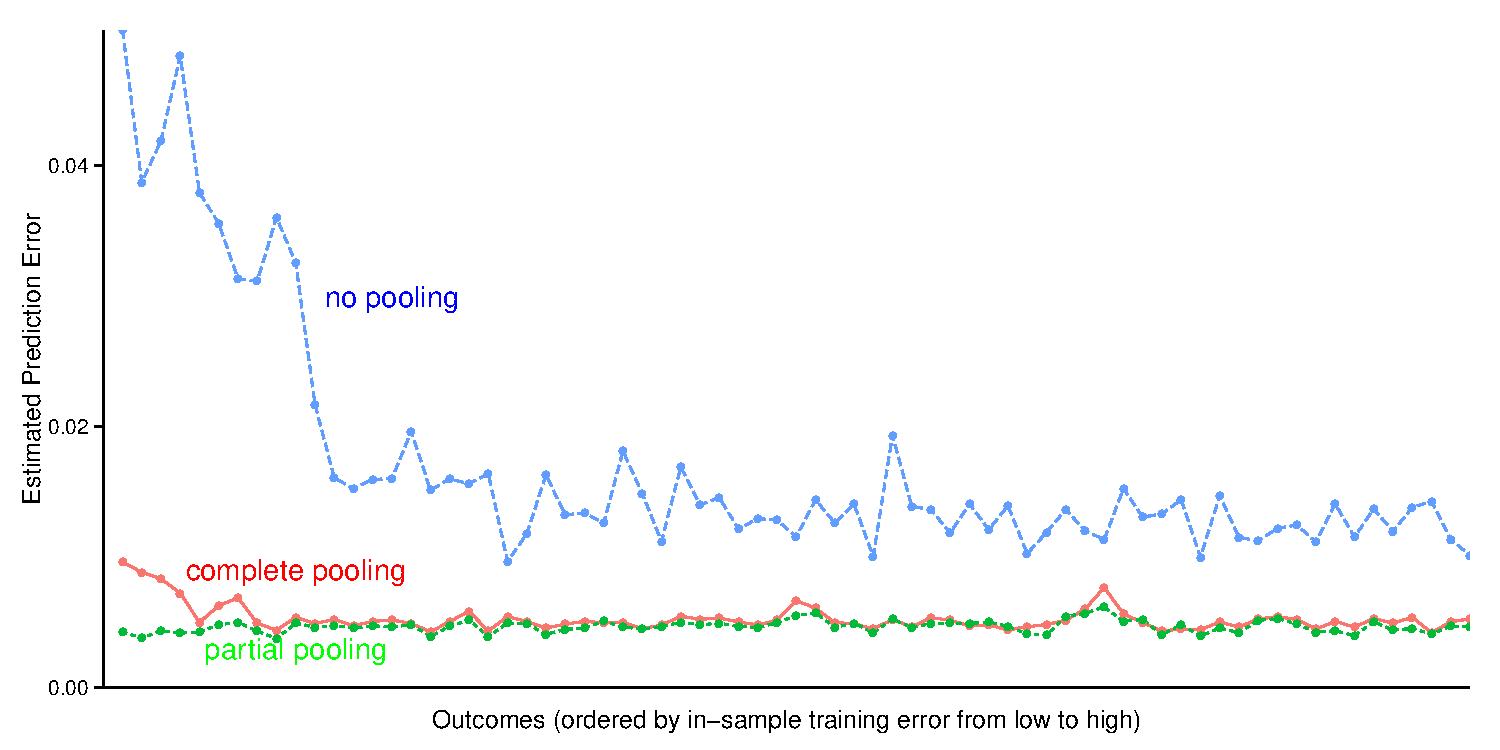
\includegraphics[width=.85\textwidth]{alloutcomesx1.pdf}
  \caption{\em Measure of fit (estimated prediction error) for all response outcomes
    in the 2006 Cooperative Congressional Election Survey. Outcomes are ordered by the lower bound
    (in-sample loss of the saturated model). The no pooling model
    gives a bad fit.  Partial pooling does best but in most cases is almost indistinguishable from complete pooling under the cross-validation criterion.}
  \label{fig:figx1}
\end{figure*}

We begin by estimating the prediction errors of all outcomes in the survey. The
results are shown in Figure~\ref{fig:figx1}. The $x$-axis is ordered by the
in-sample training loss of the saturated model $TL(M_{\text{s}},D)$, which we use
as a surrogate for a lower bound of predictive
loss. % Heuristically, for outcomes that have
% smaller lower bound of predictive loss, the more we can get from modeling,
% i.e., less divided opinion and stronger demographic variations.
For complete pooling and partial pooling, the prediction error stays stable
across different outcomes, while the no pooling model has huge prediction error
for outcomes with small lower bounds. This finding makes sense since these are
the settings where overfitting is most severe (saturated models achieve the lowest
in-sample training error). However, the difference in prediction error between
complete pooling and partial pooling seems negligible. Partial pooling is giving
essentially the same result as complete pooling, at least according to
cross-validation on individual survey responses.

\begin{figure*}
  \centering
  \subfigure{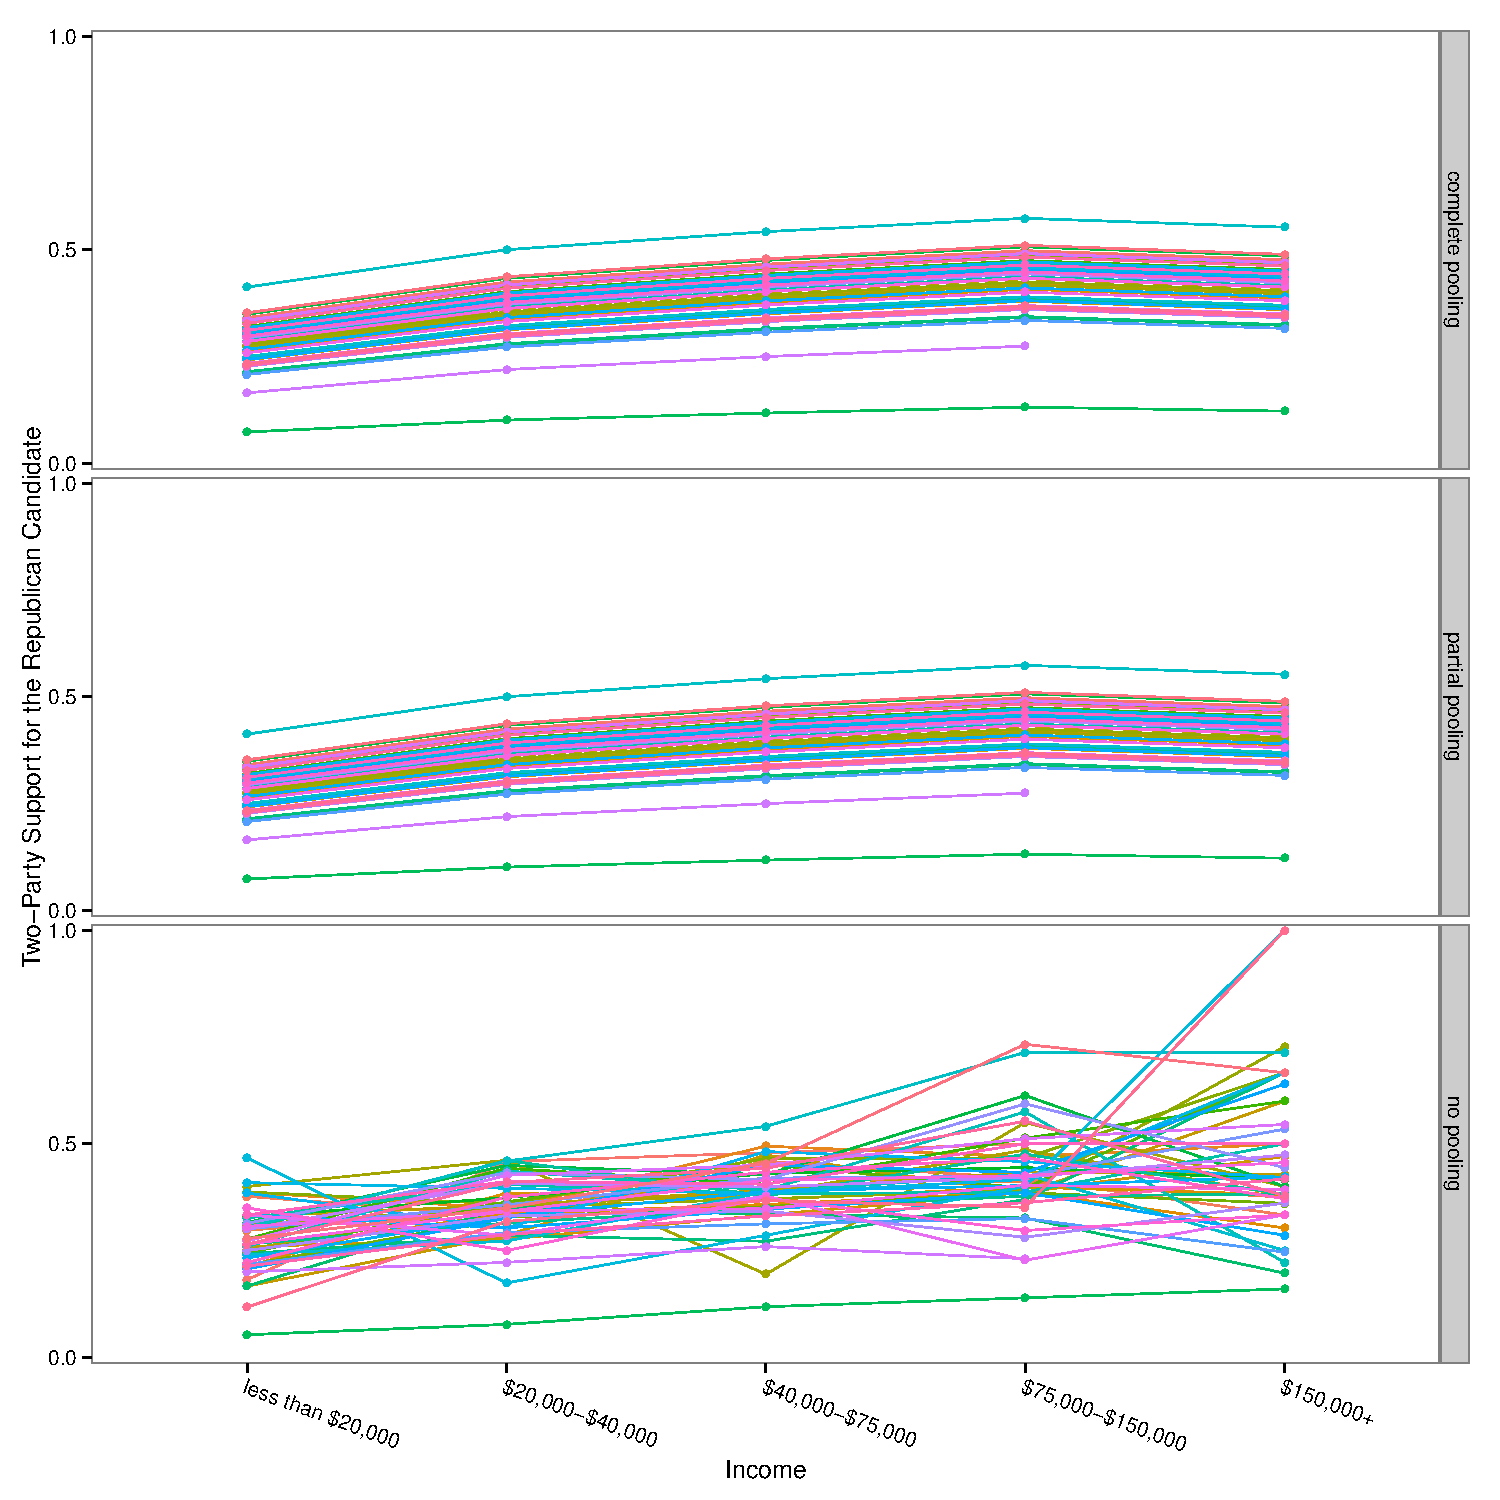
\includegraphics[width=.4\textwidth]{esti_all_bglmer}}
  \subfigure{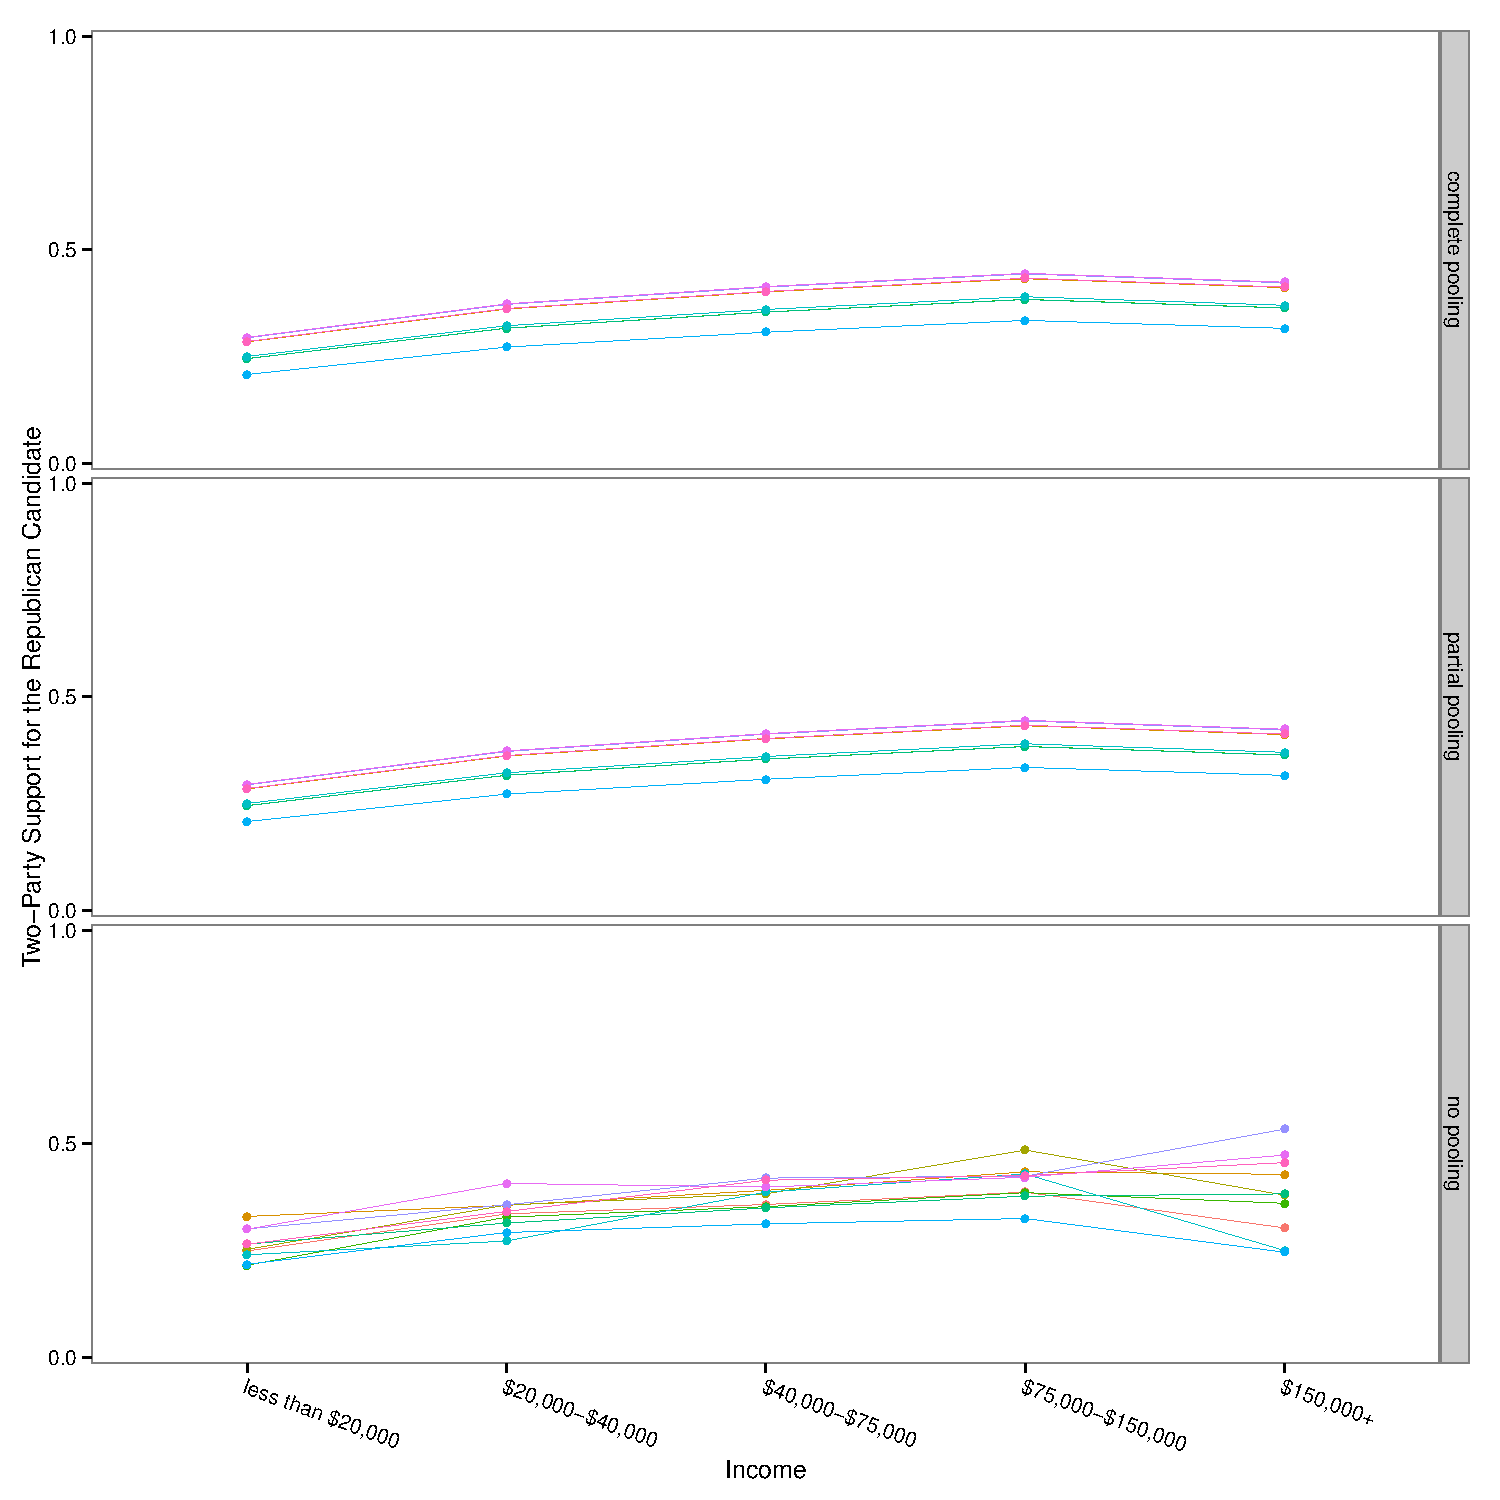
\includegraphics[width=.4\textwidth]{esti_big_bglmer}}
  \caption{\em Left panel: Cell proportion estimates for three models of vote
    intention. Each line is a state. The
    partial pooling model pools so much that it is indistinguishable from
    complete pooling. Right panel: The same estimates for the 10 most populous
    states. Still, partial pooling estimates are similar to complete pooling
    estimates.}
  \label{fig:234}
\end{figure*}

This seems to suggest that partial pooling does not have enough information to
estimate cell-to-cell variation, thus giving an overly conservative
estimate. Indeed, when we plot the estimates of $\pi_{j_1j_2}$ for one particular
outcome, vote preference for in the congressional election (see the left panel of
Figure~\ref{fig:234}), the estimates from partial pooling are almost identical to
those from complete pooling. Even for populous states where, because of their
large sample size, the amount of partial pooling should be small, there are no
major differences between estimates from partial pooling model and estimates from
complete pooling model (see the right panel of Figure~\ref{fig:234}). This
pattern is consistent across different outcomes.

Although we believe partial pooling is intrinsically better than complete
pooling, it seems that the given data are not sufficient for the partial pooling
model to pick up the interaction and unpool the estimates appropriately. It is a
result of the particular characteristics of this data set?  There are three
factors determining the structure of the data that might affect the extent of
pooling of the model. First is the sample size. If we increase the sample size to
a sufficiently large level, the partial pooling model will be able to partially
pool the estimates to an appropriate amount. As sample size grows, the no pooling
model will eventually have the same performance as partial pooling, and it might
be interesting to see at what point the saturated model becomes acceptable. The
second factor affecting the relative performance of the different models is the
size of the interactions that are being estimated, and the third factor is the
level of imbalance in the hierarchical structure. Survey data classified by
demographic and geographic predictors are typically highly unbalanced due to the
long tails of sizes typical in taxonomic structures \citep{Mandelbrot:1955}. For
example, the 2006 CCES includes 3,637 respondents from California but only 131
from Arkansas. This unbalanced structure will affect the amount of pooling
performed by a multilevel model.

In the following subsections, we conduct simulations that vary sample size and
the structure of the cells to investigate how these factors affect the relative
performance of the three models as captured by cross-validation.

\subsection{How Sample Size Changes the Dynamics}
\begin{figure}[p]
  \centering
  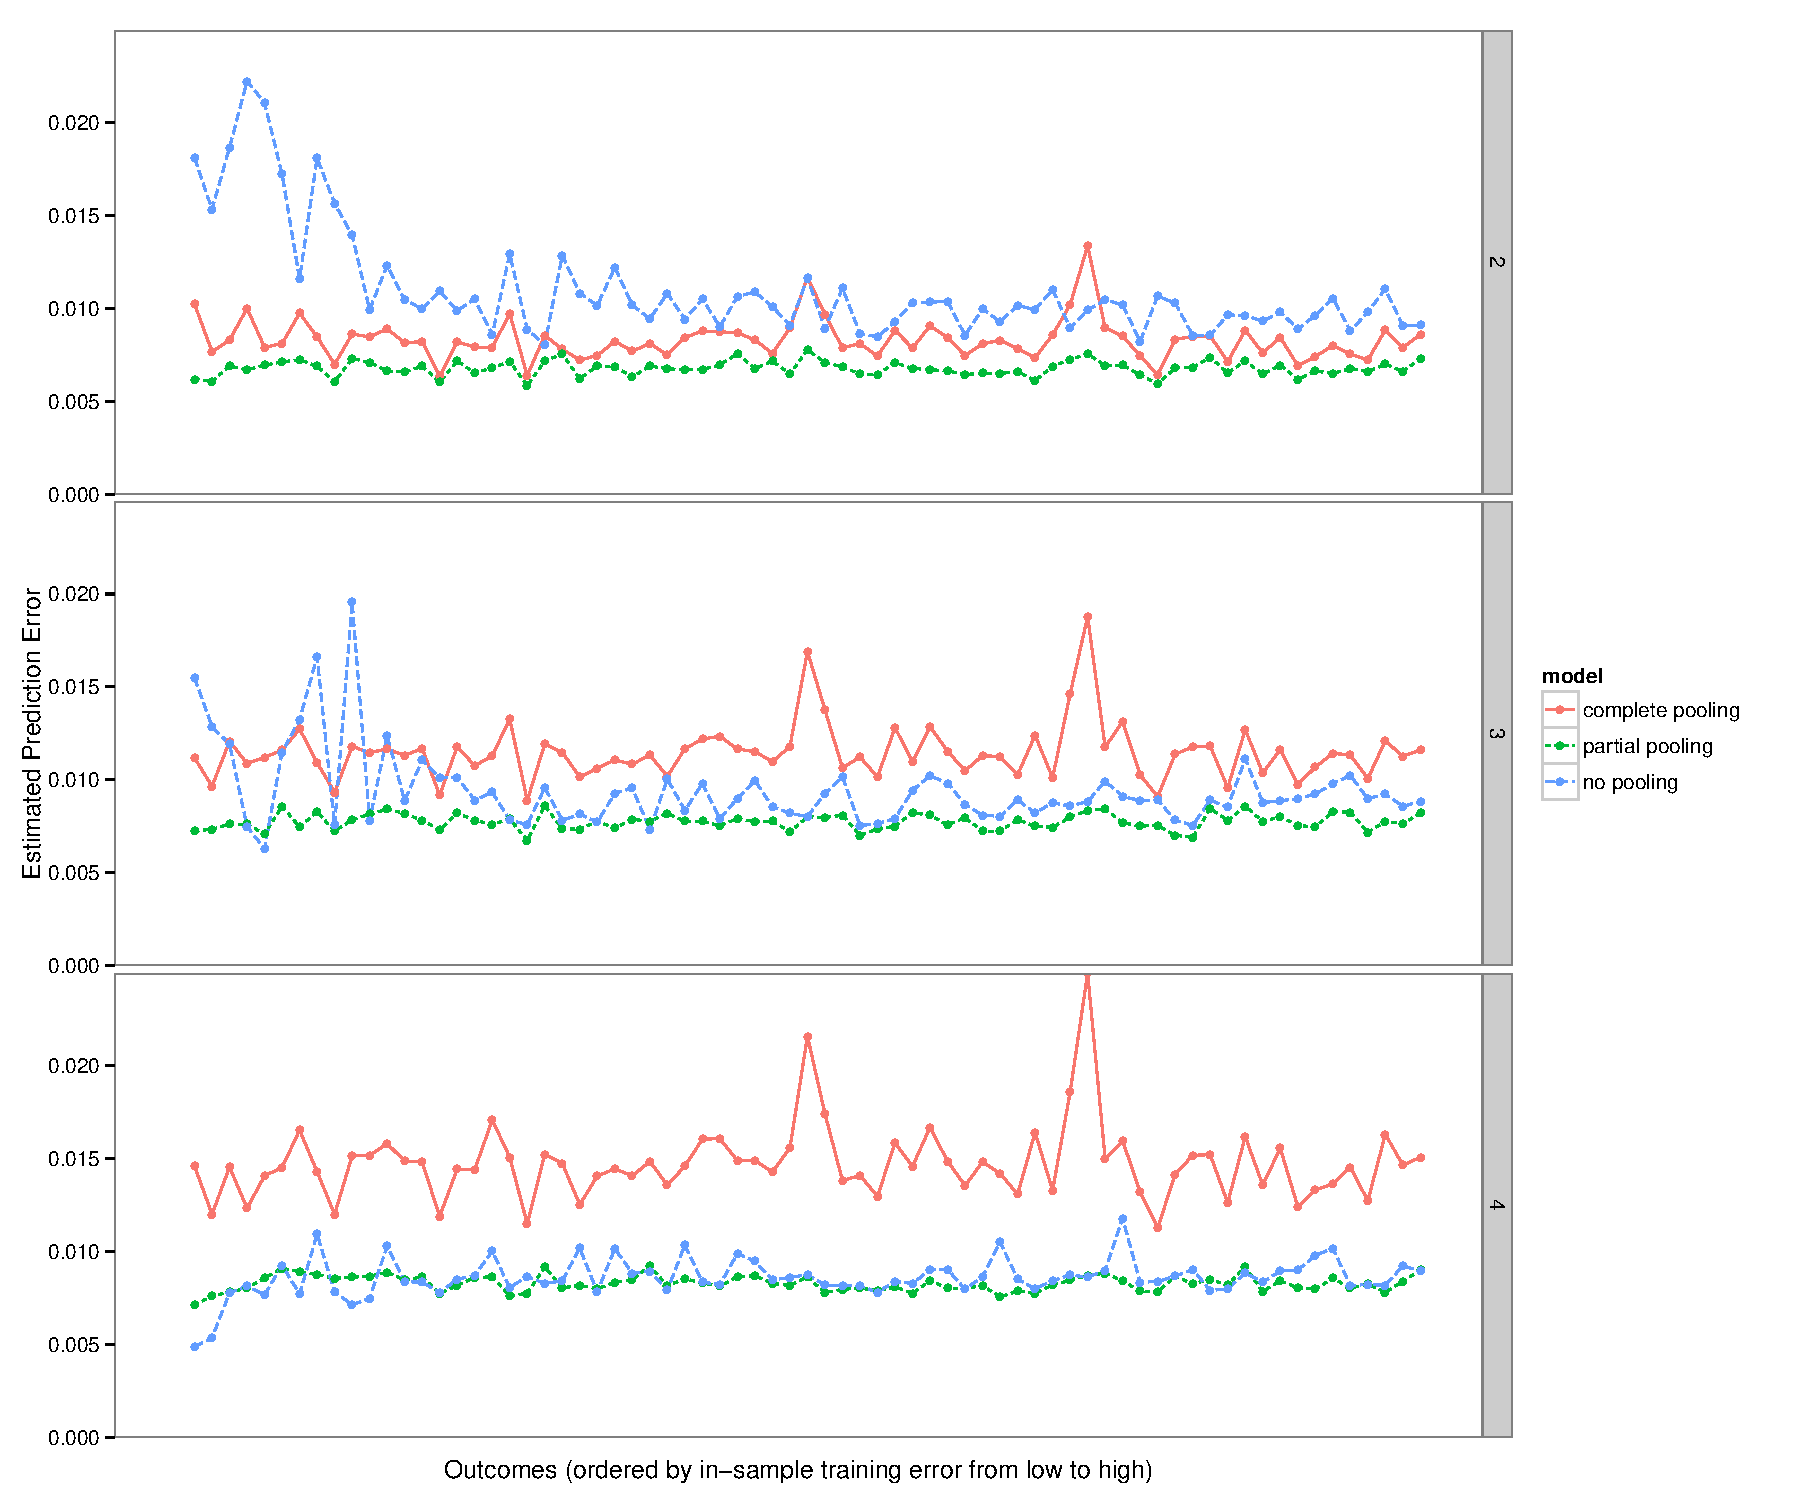
\includegraphics[width=.45\textwidth]{outcome234.pdf}
  \caption{\em Estimated prediction error of all response outcomes for augmented
    data sets. From top to bottom, the data sets have 2, 3, and 4 times as many
    data points as the original data set. The outcomes are ordered by the
    in-sample predictive loss. As sample size grows, complete pooling
    gradually gets worse and no pooling gets better.}
  \label{fig:figx234}
\end{figure} 
We artificially augment the data set by combining the data set with itself. New
data sets with sample size that are 2, 3 and 4 times as large are generated.
This augmentation still maintains the same level of interactions and cell
structure as those of the original data. Then we estimate the prediction errors
for all outcomes for the three models. Results are plotted in
Figure~\ref{fig:figx234}. As we expected, as sample size grows, the prediction
error of complete pooling model, which is essentially a wrong model, dominates
the other two; while the prediction error of no pooling model keeps
decreasing. When the sample size is 4 times as large as the original data set, no
pooling model has almost the same prediction error as partial pooling model. This
makes sense, since the problem of overfitting eventual goes away if we have
sufficiently large sample size and fixed model structure.
\begin{figure*}
  \centering
  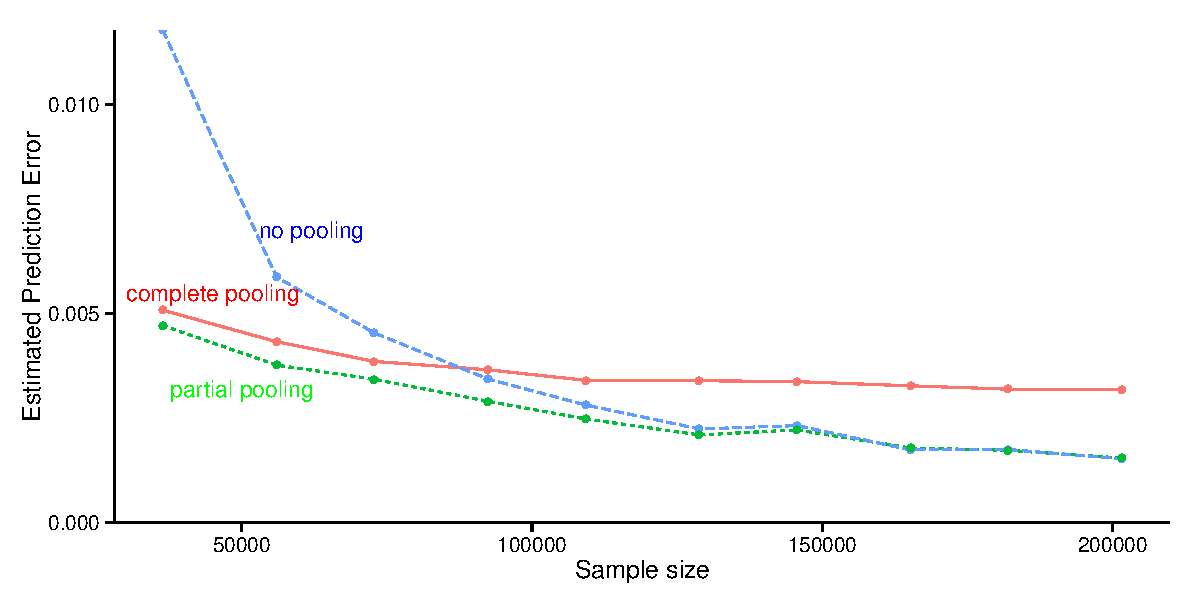
\includegraphics[width=.85\textwidth]{hourvote.pdf}
  \caption{\em Prediction error of the three models as sample size grows. The
    outcome under consideration is partisan vote preference in the upcoming
    congressional election. By this criterion, partial pooling and complete
    pooling perform similarly until sample size exceeds 50,000.}
  \label{fig:hourvote}
\end{figure*}

These results suggest that for a fixed data structure, partial pooling decisively
outperforms no pooling and complete pooling only for a certain window of sample
sizes. To have a closer look at the range of the window, we look at one
particular outcome, the vote preference in the upcoming election for the
U.S. House of Representatives. We augment the sample size and plot the relative
performance of the three models in Figure~\ref{fig:hourvote}. Partial pooling
model is noticeably better than complete pooling in this setup when the total
sample size exceeds larger than 50,000. Other outcomes have similar patterns.


\subsection{Balancedness of the Hierarchical Structure}


One possible explanation for the steep learning curve of the partial pooling
model is the highly unbalanced structure of the data. Although we have 50 states,
the estimate of the covariance of the state random effects might not be reliable
since some of the states have small sample sizes. To see how the balancedness of
the structure affects the model, we simulate a data set based on partial pooling
estimates from the original data set, but make each demographic-geographic cells
of roughly the same size. The overall sample size is the same as that of the real
data. Relative performance of the three models for all outcomes is plotted in
Figure~\ref{fig:figbal}. The graph shows that with balanced hierarchical
structure, at the same sample size and amount of interaction, partial pooling
kicks in much more quickly. Thus partial pooling is consistently better than
complete pooling in this scenario. As in the previous analysis, we also look at
the relative performance of the three models as sample size grows. The results
are plotted in Figure~\ref{fig:hourvote_bal}.

\begin{figure}[h]
  \centering
  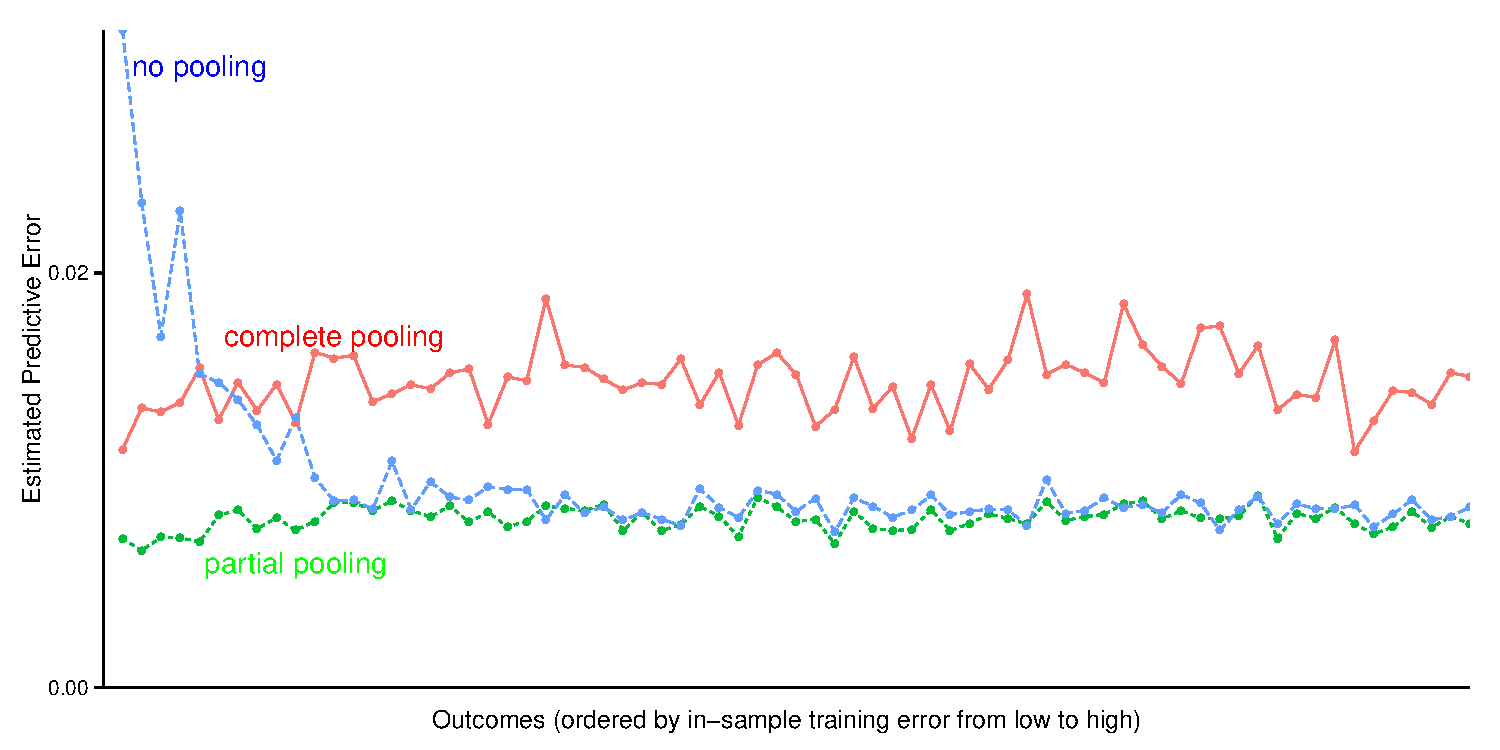
\includegraphics[width=.45\textwidth]{alloutcomesxbal.pdf}
  \caption{\em Measure of fit (prediction error) for all outcomes, ordered by
    in-sample training loss. The data set is simulated from real data set, and
    has the same sample size in total as the real data set, but keeping all
    demographic-geographic cells balanced. In this case, complete pooling model
    has much higher prediction errors than no pooling and partial
    pooling. Partial pooling is slightly but consistently better than no
    pooling. In particular, no pooling model has huge prediction error for
    outcomes that have smaller in-sample training loss.}
  \label{fig:figbal}
\end{figure}


\begin{figure}[h]
  \centering
  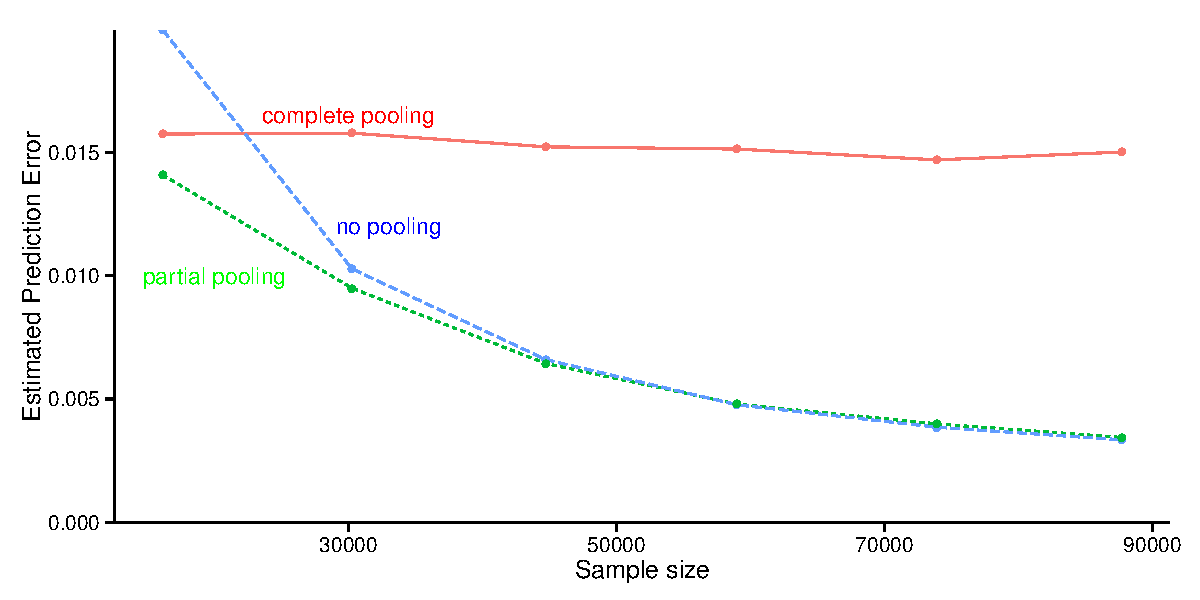
\includegraphics[width=.45\textwidth]{hourvote_bal.pdf}
  \caption{\em Prediction error of the three models as sample size grows under the
    simulated balanced data set. The outcome under consideration is the vote for
    the Republican candidate in the U.S House of Representatives. Partial
    pooling has the lowest prediction error when sample size is under 70,000.}
  \label{fig:hourvote_bal}
\end{figure} 


% As we have discussed in section~\ref{subsec:relative}, the advantage of Multilevel model is
% not absolute. From a Bayesian perspective, the prediction error is
% conditioned on available sample size and true data generating process. If we
% have infinite data, then the overfitting Interaction model will have the same
% prediction error as Multilevel model. On the other hand, if the sample size
% is Small, then the Multilevel model cannot capture the interaction between state
% and income, and thus be similar to the additive model. If we mentally plot a
% graph of relative performance of the three models, then we suspect we are in the
% left tail of the sample size graph. We want to complete this plot.



\section{Discussion}
Cross-validation is an important tool used to evaluate a wide variety of
statistical methods and has been widely used in model comparison when predictive
power is of concern. Some theoretical treatments have pointed out situations
where cross-validation might have problems. For example, \citet{shao1993linear}
shows that, under the frequentist setting, using leave-one-out cross-validation for
linear model variable selection is not consistent. % For a
% good survey of cross-validation in frequentist setting, see
% \citet{arlot2010survey}.
However, the simplicity and transparency of cross-validation gives it a near-universal
appeal. In this paper, we investigate the
sensitivity of cross-validation as a model comparison instrument in a
cross-tabulated multilevel survey data set.

We set up the model selection problem, considering three models for these structured data:  the classical models of complete pooling and no pooling,
and a Bayesian multilevel model.  The multilevel
model captures important interactions that are not included in the complete
pooling model, while at the same time avoiding the inevitable overfitting from
the no pooling model. However, the improvement of the multilevel model as given
by cross-validation is surprisingly tiny, almost negligible to unsuspecting eyes.
The problem is that improved fits with binary data yield minuscule improvements
in log loss, in moderate sample sizes nearly indistinguishable from noise even if
the improved estimates are substantively important when aggregated (for example,
state-level public opinion).  Simulations based on real data show that
sample size and structure of the cross-tabulated cells play important roles in
the relative margins of different models in cross-validation based model
selection. Caution should be exercised in applying prediction error for model
selection with structured data.
\section*{Acknowledgements}
We would like to thank the two anonymous reviewers for constructive comments.

\bibliographystyle{imsart-nameyear}
\bibliography{crossval}

\end{document}
